\chapter{Verwendete Technologien}\label{cha:theoretical-background}
\section{Entity Framework}
Zum Nutzen einer Datenbank in Programmen gibt es das von Microsoft entwickelte Entity Framework. Dabei handelt es sich um ein Framework zur Erstellung von objektrelationalen Abbildungen auf .NET-Objektstrukturen. Das wird auch als ORM (object relational mapping) bezeichnet. In anderen Worten ermöglicht es Programmieren in der Applikation mit Objekten zu arbeiten, anstatt sich auf die wirkliche Datenbank mit ihren Tabellen und den Zugriff darauf konzentrieren zu müssen. Der Grund der Notwendigkeit eines solchen Frameworks ist, dass objektorientierte Programmiersprachen wie .NET Daten in Objekten speichern und relationale Datenbanken Daten in Tabellen ablegen. Diese beiden Arten der Speicherung sind grundlegend verschieden, weshalb ein Framework benötigt wird um diese miteinander verwenden zu können.
\begin{figure}[H]
\begin{center}
	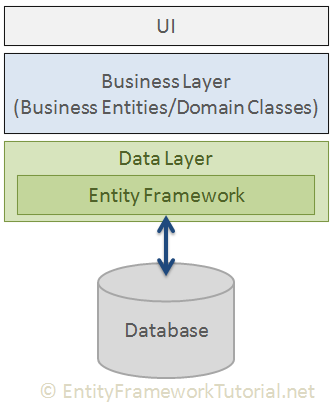
\includegraphics[scale=.65]{images/ef.png}
\end{center}
	\caption{Einsatz des Entity Frameworks in einer Applikation}
	\label{fig:sample}
\end{figure}
\noindent Wie man in der obenstehenden Grafik erkennen kann, verbindet das Entity Framework die Objekte im Programm mit der Datenbank. Dabei kann es Daten von Properties in  Objekten in die Datenbank speichern und umgekehrt Daten von der Datenbank in Objekte verwandeln. \newline
Um eine Datenbank zu verwenden, gibt es drei Möglichkeiten:
\begin{itemize}
\item Code First: Dabei werden die benötigten Klassen im Programm zuerst definiert und darauf basierend wird vom DbContext die Datenbank erzeugt. Diese Methode wurde gewählt um die Datenbank dieser Arbeit zu erstellen.
\item Model First: Im Gegensatz zu Code First werden hier zuerst die Entitäten der Datenbank mit Hilfe eines grafischen Tools modelliert und darauf basierend wird ein Datenbankschema erstellt.
\item Database First: Es wird eine bestehende Datenbank verwendet.
\end{itemize}
Zum Verwenden der Datenbank wird im Programm eine Klasse erzeugt, die von der Klasse ''DbContext'' abgeleitet wird. Diese Klasse enthält DbSets aller Entitätsklassen und gibt mittels des Connectionstrings an, welche Datenbankverbindung verwendet werden soll. Das ist sehr nützlich, weil damit die Datenbank sehr einfach ausgetauscht werden kann. Ein DbSet ist eine Klasse, die die entsprechenden Methoden für Entitätstypen anbietet (Zum Beispiel 'Add' oder 'Remove'). \newline Beispielsweise werden so alle Kunden der Datenbank verwaltet: 
\begin{lstlisting}
public DbSet<Customer> Customers { get; set; }
\end{lstlisting}
Mit dieser Property kann nun im Programm gearbeitet werden. Das heißt, dass alles was in diesem DbSet geändert wird, mit der Methode ''SaveChanges'' (aufgerufen vom  DbContext) auch in die entsprechende Tabelle in der Datenbank übertragen wird. Wenn zum Beispiel ein Objekt Customer an das DbSet Customers angehängt wird, und dann ''SaveChanges'' aufgerufen wird, wird auch in der Datenbank ein neuer Datensatz erstellt. Somit lässt das Entity Framework zu, dass Insert-, Update- oder Delete-Statements auf der Datenbank ausgeführt werden.
Zum Holen von Daten aus der Datenbank kann der Programmierer die Abfragesprache Linq benutzen. Dabei übersetzt das Entity Framework das jeweilige Linq-Statement in die Abfragesprache der verwendeten Datenbank (z.B. SQL). Über sogenannte ''DataAnnotations'' können mittels des Entity Frameworks auch Bedienungen festgelegt werden, welche gewisse Spalten von Entitäten in der Datenbank erfüllen müssen. Zum Beispiel wird mittels der Data-Annotation ''MaxLength'' festgelegt, dass der Name eines Ortes nicht länger als 100 Zeichen sein darf:
\begin{lstlisting}
[MaxLength(100)]
public string TownName { get; set; }
\end{lstlisting}
Quellen: \cite{wikipedia_entity_2017}, \cite{entityframework_tutorial_what_2018}, \cite{wikipedia_objektrelationale_2016}, \cite{microsoft_entity_connections_2018}, \cite{microsoft_entity_2018}
\subsection{Linq}
Linq steht abgekürzt für Language Integrated Query und ermöglicht den Zugriff auf Daten aus einem Programm. Mit dieser Abfragesprache kann der Benutzer auf lokale Listen im Programm zugreifen, auf Daten aus der Datenbank, auf XML-Inhalte und vieles mehr. Im Falle dieser Arbeit wird aber nur Linq to Objects und Linq to Entities verwendet. Linq to Entites ermöglicht dem Programmierer im Code direkt Abfragen an das konzeptionelle Modell vom Entity Framework zu stellen. Genauer gesagt werden diese Abfragen dann in Befehlsstrukturen umgewandelt und dann gegen den Objektkontext ausgeführt.
\newline Linq hat die Eigenschaft, dass die gegebenen Ausdrücke nicht bei ihrer Definition ausgeführt werden, sondern erst wenn der Wert tatsächlich gebraucht wird (Lazy Evaluation). Das hat zum Vorteil, dass Abfragen öfter verwendet werden können. Falls der Benutzer das nicht möchte, muss er vortäuschen, die Ergebnismenge sofort zu benötigen (zum Beispiel kann nach der Query ein .ToList() angehängt werden).
\newline Mit der nachfolgenden Codezeile werden beispielsweise alle Kontaktlinsenaufträge gewählt, die schon bezahlt wurden.
\begin{lstlisting}
List<Order> paidContactLenses = this.ContactLenses.Where(c => c.PaymentState == "Bezahlt").ToList();
\end{lstlisting}
Ein anderes Beispiel wäre alle Kunden zu zählen, deren Vorname mit 'E' beginnt:
\begin{lstlisting}
int customersStartingFirstNameWithE = this.Customers.Count(c => c.FirstName.StartsWith("E"));
\end{lstlisting}
Quellen: \cite{wikipedia_linq_2018}, \cite{microsoft_linq_2018}
\section{UnitOfWork-Pattern}
Das UnitOfWork-Pattern ist eines von vielen Design Patterns in .NET. Design Patterns sind allgemeine Lösungen für Software Design Probleme, die immer wieder vorkommen. Das UnitOfWork-Pattern beschreibt einen Weg der Projektarchitektur um mit Datenbanken arbeiten zu können. Es verwaltet Transaktionen, führt Updates geregelt durch und schafft damit Concurrency-Probleme aus der Welt. Dadurch arbeitet man im Code nicht direkt mit den DbSets sondern mit der Klasse UnitOfWork. \newline Genauer gesagt, muss der Programmierer zuerst das Repository-Pattern implementieren, um das UnitOfWork-Pattern umzusetzen zu können. Dabei geht es nur darum, für jede Entität eine Klasse zu erschaffen (Repository), die alle Operationen für diese Entität beinhaltet. In einem Repository für die Klasse Kunde sollten zum Beispiel die CRUD Methoden (Create, Read, Update, Delete) enthalten sein. In dieser Arbeit wurde das Pattern umgesetzt, indem eine generische Klasse ''GenericRepository'' für alle Entitäten gestaltet wurde (siehe Data-Access-Layer). 
\newline Mit dem Repository-Pattern alleine (ohne UnitOfWork-Pattern), enthält jedes Repository einen eigenen DbContext, welche nicht aufeinander abgestimmt sind. Das würde allerdings zu Problemen führen, besonders wenn zwei verschiedene Repositories eingesetzt werden und beide gleichzeitig Transaktionen abschließen. Jedes Repository hätte dann seine eigene Version von eventuell geänderten Datensätzen, sich vielleicht unterscheiden würden. Das würde letztendlich zur Datenbankinkonsistenz führen.
\newline Um dieses Problem zu vermeiden, wird das UnitOfWork-Pattern eingesetzt. Dabei wird eine Klasse ''UnitOfWork'' erstellt, die eine Instanz von allen Repositories enthält und einen zentralen DbContext, der an die einzelnen Repositories weitergegeben wird. Damit können nun Datenbankänderungen, in denen mehrere Repositories benötigt werden, gesammelt in 
einer Transaktion auf einem zentralen DbContext ausgeführt werden.
\newline
\newline
\underline{Data-Access-Layer:}
In dieser Arbeit wurde das Repository Pattern und das UnitOfWork-Pattern mit folgenden Klassen implementiert:
\begin{itemize}
\item EntityObject: Dies ist eine Klasse, von der später alle Entitäten ableiten. Sie gibt den Entitäten eine Id und einen Timestamp, um später Concurrency-Probleme zu lösen.
\item IGenericRepository: Ein Interface für alle Repositories, welches die Standardmethoden wie Get, Insert oder Delete vorschreibt.
\item IUnitOfWork: Ein Interface, welches die Definitionen für alle IGenericRepositories, die Save-Methode sowie andere Methodenköpfe, die später selbst implementiert werden, enthält.
\item GenericRepository: Eine Klasse, die für jede Entität erstellt wird und die von IGenericRepository ableitet. Sie enthält den Context sowie das DbSet der gewünschten Entität. Zusätzlich implementiert sie alle Standardmethoden (Get, GetById, Insert, Update, Delete, Count...).
\item UnitOfWork: Eine Klasse, die von IUnitOfWork ableitet und alle Methoden implementiert. Mit dieser Klasse wird später im Programm gearbeitet. 
\end{itemize}
Zum Beispiel wird mit diesem Befehl ein Kunde mittels der Id gesucht. Das globale, private Feld ''uow'' wird zuvor mittels Dependency Injection im Konstruktor initialisiert.
\begin{lstlisting}
Customer c = uow.CustomerRepository.GetById(id);
\end{lstlisting}
Es wird also zuerst auf die UnitOfWork zugegriffen und von dort aus auf das spezielle Repository. CustomerRepository ist vom Typ GenericRepository \textless Customer\textgreater  und damit kann man auf die im GenericRepository definierten Methoden (hier GetById) zugreifen.
\newline
Ein anderes Beispiel wäre das Einfügen eines neuen Datensatzes in die Datenbank. Dazu muss unbedingt die Save-Methode danach aufgerufen werden, denn sonst werden die Änderungen nicht in die Datenbank übertragen.
\begin{lstlisting}
uow.CustomerRepository.Insert(this.Customer);
uow.Save();
\end{lstlisting}
Die Klasse ''UnitOfWork'' beinhaltet auch eine Methode namens ''Dispose'' welche auf jeden Fall aufgerufen werden muss um den DbContext zu schließen.
\newline Quellen: \cite{codeproject_unit_2018}, \cite{dofactory_.net_2018}, \cite{c-sharpcorner_unit_2018}
\section{WPF}
WPF (Windows Presentation Foundation) ist eine von Microsoft entwickelte Klassenbibliothek zur Erstellung von grafischen Oberflächen. Mit WPF werden häufig Desktopanwendungen erstellt, allerdings gibt es auch die Möglichkeit 3D-Grafiken, Dokumente oder Videos zu erstellen. Als Vorgängerversion kann man Windows Forms bezeichnen, denn WPF beinhaltet weitaus mehr Möglichkeiten des Designs als Windows Forms.
Um eine WPF-Anwendung erstellen zu können, benötigt man die Definitionssprache XAML. Dies ist abgekürzt und steht für Extensible Application Markup Language. Diese Sprache basiert auf XML und beinhaltet zusätzlich WPF-spezifische Elemente. \newline Beispiel eines XAML-Codes und dessen Erscheinen: 
\begin{lstlisting}
<Window x:Class="OpticianMgr.Wpf.Pages.AddCountryWindow"
        xmlns="http://schemas.microsoft.com/winfx/2006/xaml/presentation"
        xmlns:x="http://schemas.microsoft.com/winfx/2006/xaml"
        xmlns:d="http://schemas.microsoft.com/expression/blend/2008"
        xmlns:mc="http://schemas.openxmlformats.org/markup-compatibility/2006"
        xmlns:local="clr-namespace:OpticianMgr.Wpf.Pages"
        mc:Ignorable="d"
        Title="Neues Land" Height="179.589" Width="576.437">
    <StackPanel Style="{StaticResource StackPanelBackground}">
        <Label Style="{StaticResource HeadingStyle}">Neues Land</Label>
    </StackPanel>
</Window>
\end{lstlisting}
\begin{figure}[H]
\begin{center}
	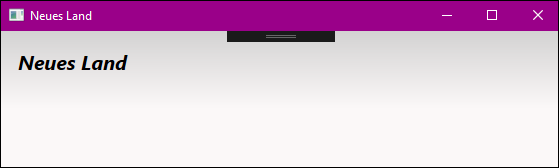
\includegraphics[scale=.6]{images/Wpf.png}
\end{center}
	\caption{Einfaches WPF-Fenster}
	\label{fig:sample}
\end{figure}
Dennoch hat WPF auch manche Nachteile:
\begin{itemize}
\item WPF benötigt ein jüngeres Betriebssystem als Windows XP.
\item Es kommt zu Leistungsproblemen, wenn mehrere Fenster im Einsatz sind und außerdem hat WPF einen hohen RAM-Bedarf.
\end{itemize}
Quellen: \cite{it-visions_was_2018}, \cite{schwichtenberg_vor-_2018}
\section{MVVM}
MVVM ist eine Abkürzung und steht für Model-View-ViewModel. Dies ist ein Entwurfsmuster, wie man Projekte designen kann und dient zur Trennung der Logik und der Darstellung der Benutzerschnittstelle. Es ist speziell geeignet für WPF. 
\begin{figure}[H]
\begin{center}
	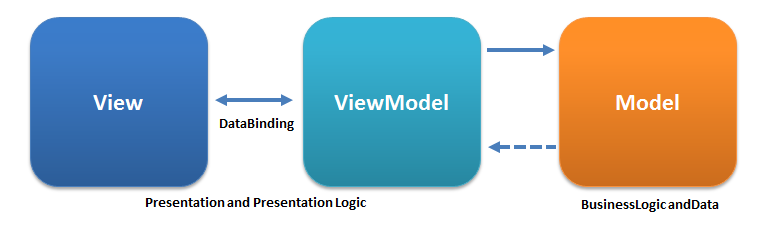
\includegraphics[scale=.7]{images/MVVMPattern.png}
\end{center}
	\caption{MVVM-Konzept}
	\label{fig:sample}
\end{figure}
\noindent In der obenstehenden Grafik kann man leicht erkennen, wie MVVM funktioniert. Die View kommuniziert ausschließlich mit dem ViewModel und zwar über DataBindings. Das ViewModel beinhaltet die Logik und verändert gegebenenfalls das Model (Datenbank).
\newline
DataBindings von dem ViewModel zur View funktionieren mit Hilfe des Events ''PropertyChangedEventHandler''. 
\begin {lstlisting}
public event PropertyChangedEventHandler PropertyChanged;
\end{lstlisting}
Mit der Methode ''Invoke'' wird das Event ausgelöst. Es benachrichtigt die View, dass sich der Wert der Property mit dem Namen ''propertyName'' geändert hat. Im ersten Parameter wird der Sender des Events übermittelt. In diesem Fall ist der Sender das ViewModel (this), in dem das Event ausgelöst wird.
\begin{lstlisting}
PropertyChanged?.Invoke(this, new PropertyChangedEventArgs(propertyName));
\end{lstlisting}
Im Gegenzug kann die View folgendermaßen auf eine Property im ViewModel binden:
\begin{lstlisting}
<ListView ItemsSource="{Binding CustomersView, Mode=TwoWay, UpdateSourceTrigger=PropertyChanged}">
\end{lstlisting} \newpage
Vorteile von MVVM:
\begin{itemize}
\item Logik sowie Darstellung können unabhängig voneinander bearbeitet werden. Dadurch kann die Darstellung von Designern und die Logik von Entwicklern erstellt werden.
\item Durch die Trennung ergibt sich eine bessere Testbarkeit der Logik.
\end{itemize}
Quellen: \cite{wikipedia_model_2017}
\section{MVVM-Light}
MVVM-Light ist ein Framework, welches dazu dient, den Aufwand der Implementierung des MVVM-Musters zu verringern. Neben MVVM-Light gibt es auch noch andere solcher Frameworks, wie zum Beispiel Prism. \newline Zur Verwendung müssen die Packages MVVMLight (Version 5.3.0) und MVVMLightLibs (Version 5.3.0) über den NuGet-Package-Manager installiert werden. \newline Beim Einbinden von MVVM-Light werden zwei wesentliche Klassen erstellt
\begin{itemize}
\item MainViewModel: Das ViewModel der Hauptseite, abgeleitet von der Klasse ''ViewModelBase''.
\item ViewModelLocator: Beinhaltet statische Referenzen für alle anderen ViewModels. Außerdem bietet diese Klasse einen einfachen IOC-Container.
\end{itemize}
Alle ViewModels, die später erstellt werden, sollten von der Klasse ''ViewModelBase'' abgeleitet werden. Damit hat der Programmierer unter anderem die Möglichkeit die Methode ''RaisePropertyChanged'' zu verwenden. Diese ermöglicht dem ViewModel die View zu benachrichtigen, dass sich Werte von Properties verändert haben und somit kann die View die entsprechenden Daten aktualisieren. \newline
Hier werden die Werte der Kundenübersicht vom ViewModel aus aktualisiert.
\begin{lstlisting}
this.RaisePropertyChanged(() => this.CustomersView);
\end{lstlisting}
MVVM-Light bietet die vorgefertigte Klasse ''RelayCommand'', welche die Implementierung des Interfaces ''ICommand'' für MVVM-Light darstellt. Der Konstruktor der Klasse hat zwei Parameter. Der erste beschreibt die Aktivität, die ausgeführt werden soll, sobald das RelayCommand aufgerufen wird (Lambda-Expression oder Delegate für Methode). Der zweite Parameter ist optional und erwartet ein Delegate für eine Methode oder eine Lambda-Expression, die ein ''bool'' zurückgibt. Dieser  beschreibt, ob das RelayCommand zur Zeit ausgeführt werden darf oder nicht.
\newline 
Im nachfolgenden Beispiel wird ein RelayCommand aufgerufen, sobald ein Button gedrückt wird.
\newline In der View wird der Name des RelayCommands im Button angegeben.
\begin{lstlisting}
<Button Command="{Binding DeleteFilter}">Filter zuruecksetzen</Button>
\end{lstlisting}
\newpage \noindent Im ViewModel wird das gewünschte RelayCommand so initialisiert:
\begin{lstlisting}
DeleteFilter = new RelayCommand(DeleteF);
\end{lstlisting}
DeleteF ist dabei die Methode, die ausgeführt wird, sobald der Button gedrückt wird. \newline Ein weiteres Feature von MVVM-Light heißt ''EventToCommand''. Dabei können alle beliebigen Events aus der View an das ViewModel in RelayCommands weitergegeben werden und dort bearbeitet werden. Zusätzlich können auch die Parameter des Events in das ViewModel übertragen werden. Das geschieht, indem der Programmieren ''PassEventArgsToCommand'' auf ''true'' setzt. Zur Implementierung müssen in der View zwei Namespaces deklariert werden:
\begin{lstlisting}
xmlns:i="clr-namespace:System.Windows.Interactivity;
assembly=System.Windows.Interactivity"
xmlns:cmd="clr-namespace:GalaSoft.MvvmLight.Command;
assembly=GalaSoft.MvvmLight.Platform"
\end{lstlisting}
Im nachfolgenden Codeabschnitt wird das Event ''Loaded'' vom RelayCommand ''Initialized'' abonniert.
\begin{lstlisting}
<i:Interaction.Triggers>
	<i:EventTrigger EventName="Loaded">
		<cmd:EventToCommand Command="{Binding Initialized}" PassEventArgsToCommand="True"></cmd:EventToCommand>
	</i:EventTrigger>
</i:Interaction.Triggers>
\end{lstlisting}
Im ViewModel kann dann auf das Event und dessen Parameter reagiert werden:
\begin{lstlisting}
public ICommand Initialized { get; set; }

public CustomerViewModel()
{
	Initialized = new RelayCommand<RoutedEventArgs>(Init);
}
private void Init(RoutedEventArgs p)
{
	//do something
}
\end{lstlisting}
Eine weiteres Feature von MVVM-Light ist der Messenger. Diese Klasse erlaubt den Austausch von Nachrichten zwischen zwei ViewModels. Die ViewModels müssen dabei keine spezielle Verbindung zueinander haben.
\newline Quellen: \cite{dotnetcurry_using_2018}, \cite{dotnetpattern_mvvm_2018}, \cite{microsoft_mvvm_2018}
\section{Microsoft Office Interop}
Um aus einem Programm Word-Dokumente zu erstellen, gibt es das Assembly Microsoft.Office.Interop.Word auf welches eine Referenz hinzugefügt wurde. Damit kann der Benutzer im Programm Word-Dokumente bearbeiten, oder Informationen aus diesen herauslesen. Zur Nutzung benötigt der Computer allerdings eine gültige Microsoft Office Lizenz.  Außerdem lädt Interop das Word-Dokument im Hintergrund, wenn es bearbeitet wird, was den ganzen Vorgang etwas langsam macht.
Dennoch bietet sich der Gebrauch von Interop an, weil es die einfachste Variante ist, auf Word-Dokumente zuzugreifen.
Im folgenden Abschnitt wird erklärt wie aus einer Vorlage ein individuelles Word-Dokument erstellt werden kann.
\begin{lstlisting}
Application wordApp = new Application();
Document wordDoc = new Document();

Object oMissing = System.Reflection.Missing.Value;
wordDoc = wordApp.Documents.Add(ref oTemplatePath, ref oMissing, ref oMissing, ref oMissing);
foreach (Field myMergeField in wordDoc.Fields)
{
	Range rngFieldCode = myMergeField.Code;
	String fieldText = rngFieldCode.Text;

	//only mergefields should be edited
	if (fieldText.StartsWith(" MERGEFIELD"))
	{
		myMergeField.Select();
		wordApp.Selection.TypeText("Test");
	}
}
wordDoc.SaveAs(completePath);
wordDoc.Close();
wordApp.Quit();
\end{lstlisting}
Über den String ''oTemplatePath'' wird der Pfad des gewünschten Templates übergeben. Danach werden alle MergeFields der Vorlage (diese kann man beim Erstellen der Vorlage einfügen: Einfügen -\textgreater Schnellbaustein -\textgreater Mergefield) mit der Zeichenkette ''Test'' ersetzt. Im Endeffekt simuliert Interop einen Klick auf das Feld und mit der Methode TypeText(''Test'') wird der Text eingefügt. Zum Abschluss wird das Dokument unter einem angegeben Pfad abgespeichert (completePath) und die geöffnete Vorlage sowie die Applikation geschlossen. \newline
Quellen: \cite{gembox_microsoft_2018}
\section{WPF-Toolkit}
Zur grafischen Darstellung der Statistiken wurde ebenfalls ein eigenes Assembly installiert:  System.Windows.Controls.DataVisualization.Toolkit (Version 4.0.0). Dieses Assembly kann einfach über den NuGetPackage-Manager heruntergeladen werden. Es ermöglicht die Veranschaulichung verschiedener Diagramme, wie zum Beispiel Linien-, Torten oder Balkendiagrammen. Zur Verwendung muss der Benutzer den Namespace in der View definieren.
\begin{lstlisting}
xmlns:toolkitCharting="clr-namespace:System.Windows.Controls.DataVisualization
.Charting;assembly=System.Windows.Controls.DataVisualization.Toolkit"
\end{lstlisting}
Im folgenden Code wird ein Liniendiagramm mit einer Linie erstellt:
\begin{lstlisting}
<toolkitCharting:Chart Title="{Binding Title}">
            <toolkitCharting:LineSeries Title="{Binding LineTitle}"  DependentValueBinding="{Binding Value}" IndependentValueBinding="{Binding Key}" ItemsSource="{Binding DataValues}"/>
</toolkitCharting:Chart>
\end{lstlisting}
In der Property ''Title'' wird der Titel des Diagramms übergeben und ''LineTitle'' beschriftet die Linie mit dem gewünschten Text. ''DataValues'' (Typ ''ObservableCollection\textless KeyValuePair\textless string, int\textgreater \textgreater'') beinhaltet die Daten, welche im Diagramm dargestellt werden sollen. ''DependentValueBinding=''\{Binding Value\}'''' beschreibt, dass die abhängigen Werte des Diagramms jeweils vom ''Value'' bezogen werden. In ''DataValues'' ist das der int. \newline
Quellen: \cite{c-sharpcorner_charting_2017}
\section{MessageBird}
MessageBird ist ein Unternehmen, welches einen Online-Dienst anbietet mit dem  Unternehmen oder auch einzelne Personen, kostenpflichtig SMS aus einem Programm versenden können. Dazu meldet sich der Benutzer auf der Website ''https://www.messagebird.com'' an und sucht sich das passende Angebot. Danach kann man sein Guthaben aufladen und bekommt im Gegenzug einen AccessKey, über den man Nachrichten versenden kann. Dabei kann jeder Benutzer von MessageBird mehrere AccessKeys haben, beispielsweise einen für Test-Nachrichten, die nicht wirklich versendet werden, oder einen AccessKey, mit dem dann echte SMS versendet werden. Für Nachrichten, die nach Österreich gesendet werden, muss der Benutzer derzeit 4,6 Cent (Stand März 2018) bezahlen. Sobald die SMS versendet wurde, wird der Betrag automatisch vom Guthaben des Benutzers abgezogen. Wenn das Guthaben aufgebraucht ist, versendet MessageBird keine SMS mehr und der Benutzer kann sein Guthaben gegebenenfalls wieder aufladen. Auf der Website hat man einen Überblick über die versendeten SMS, verschiedene angelegte Nummern und vieles mehr. \newline Über den NuGet-Manager kann man das Package ''MessageBird'' installieren und im Code dann so verwenden:
\begin{lstlisting}
IProxyConfigurationInjector proxyConfigurationInjector = null; // for no web proxies, or web proxies not requiring authentication

Client client = Client.CreateDefault(AccessKey, proxyConfigurationInjector);

MessageBird.Objects.Message message = client.SendMessage("OptikAigner", this.Message, new[] { Convert.ToInt64(this.To) });
\end{lstlisting}
''AccessKey'' im zweiten Befehl ist der String, den man von der Website bekommt, über den abgerechnet wird. ''OptikAigner'' wird als Sendernamen angegeben. Der zweite Parameter des letzten Befehls, gibt den Text der Nachricht an. Der letzte Parameter ist ein ''long''-Array mit einem Wert, nämlich der Telefonnummer, an die die SMS versendet werden soll.

\subsubsection{Andere Möglichkeiten}
Im Vergleich zum Versand von E-Mails, gibt es keine Möglichkeit kostenfrei und ohne Anbieter SMS zu versenden. Als Alternative hätte sich das Unternehmen ''Twilio'' angeboten, allerdings hätte dort eine SMS ca. 9 Cent gekostet. Aus Kostengründen und aus Benutzerfreundlichkeit ist die Wahl des Anbieters auf MessageBird gefallen.
\newline Quellen: \cite{messagebird_sms_2018}, \cite{messagebird_preise_2018}, \cite{twilio_sms_2018}